\chapter{Architettura CUDA}
\section{Cos'è CUDA}
CUDA ( Compute Unfied Device Architecture) è un architettura hardware creata da NVIDIA e pensata per l’elaborazione parallela che si basa dunque sulla suddivisione di un problema in sottoproblemi e lo svolgimento di ognuno di questi concorrentemente.
Tutto ciò è possibile sfruttando la potenza di calcolo della GPU (unità di elaborazione grafica) che assieme alla CPU permette di rendere molto efficiente in termini di tempo l’esecuzione di molte applicazioni.
Il calcolo parallelo su GPU offre prestazioni senza precedenti caricando porzioni \textbf{compute-intensive} dell'applicazione sulle GPU, mentre la porzione rimanente di codice continua ed eseguire su CPU. Pertanto, le GPU devono operare congiuntamente con le CPU mediante bus PCI-Express

\begin{figure}[H]
\centering
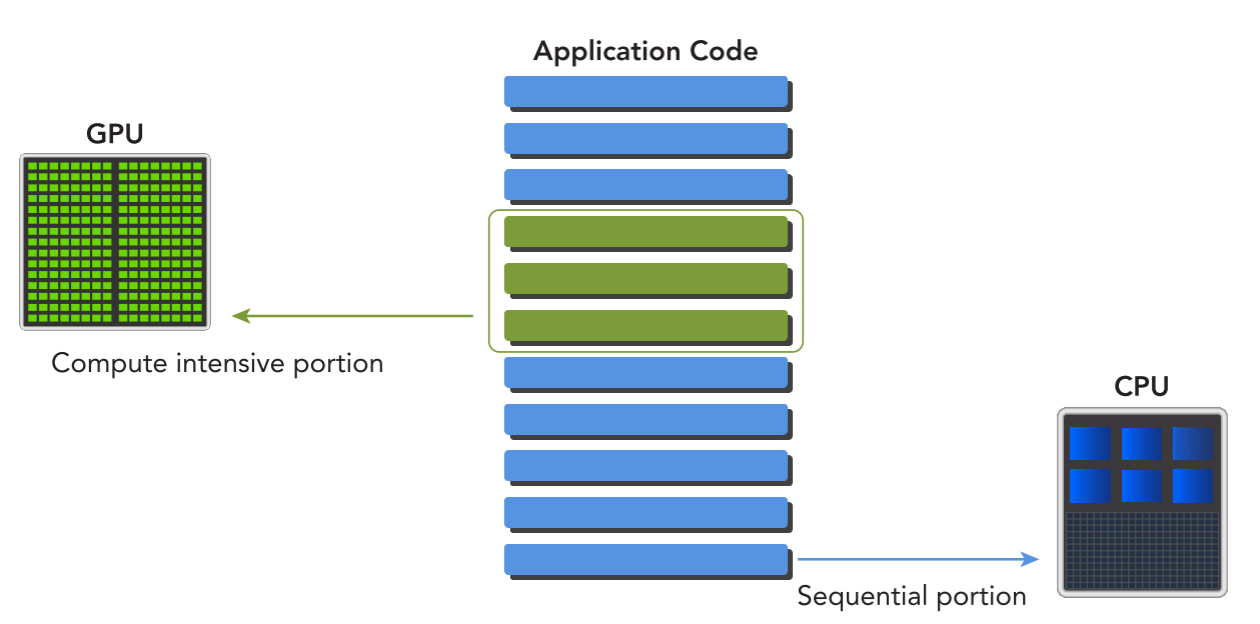
\includegraphics[scale=0.3]{img/cpu-gpu.png}
\caption{Divisione delle operazioni tra GPU e CPU in ambiente CUDA}
\end{figure}

\paragraph{}
Le applicazioni in cui CPU e GPU lavorano insieme consistono di due parti:
\begin{itemize}
\item codice Host
\item codice Device
\end{itemize}


Il codice Host esegue su \textbf{CPUs} e il codice device esegue su \textbf{GPUs}. Il codice CPU è responsabile della gestione dell'ambiente, dell'IO e della gestione dei dati per il device stesso, prima di caricare task intensivi sul device. La GPU è usata per accelerare l'esecuzione di questa porzione di codice basandosi sul parallelismo dei dati. La CPU è ottimizzata per sequenze di operazioni in cui il controllo del flusso è impredicibile; le GPU lo sono per carichi dominati da semplice flusso di controllo.

\begin{figure}[H]
\centering
\includegraphics[scale=0.3]{img/Performancecpu-gpu.png}
\caption{Prestazioni tra GPU e CPU in relazione a grado di parallelismo e quantità dei dati da elaborare.}
\end{figure}